\documentclass[border=4pt]{standalone}
\usepackage{amsmath,amssymb,tikz}
\usetikzlibrary{arrows.meta,calc,decorations.pathreplacing}
\begin{document}
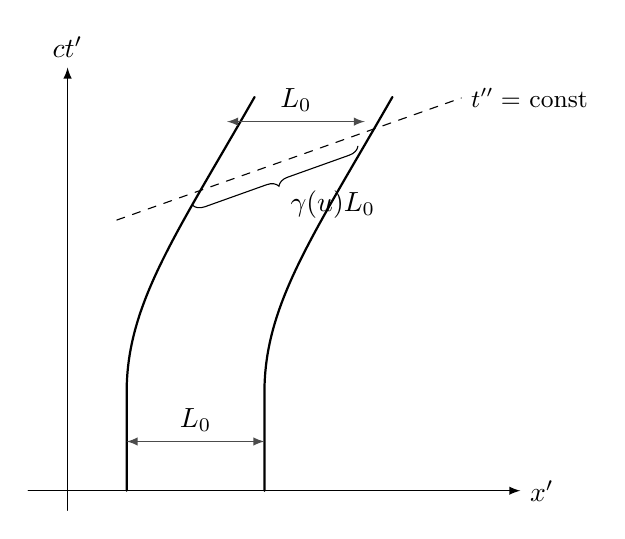
\begin{tikzpicture}[scale=1.25,>=latex,line cap=round]
  \draw[->] (-0.4,0) -- (4.6,0) node[right]{$x'$};
  \draw[->] (0,-0.2) -- (0,4.3) node[above]{$ct'$};
  % identical worldlines: rest, then hyperbolic acceleration, then uniform speed u
  \draw[thick] (0.6,0) -- (0.6,1.0) .. controls (0.6,1.9) and (1.1,2.6) .. (1.9,4.0);
  \draw[thick] (2.0,0) -- (2.0,1.0) .. controls (2.0,1.9) and (2.5,2.6) .. (3.3,4.0);
  \draw[<->,black!70] (0.6,0.5) -- (2.0,0.5) node[pos=0.5,above,black]{$L_0$};
  \draw[<->,black!70] (1.62,3.75) -- (3.02,3.75) node[pos=0.5,above,black]{$L_0$};
  % simultaneity line of S'' (slope u/c)
  \draw[dashed] (0.5,2.75) -- (4.0,3.99);
  \node[black,font=\small,anchor=west] at (4.0,3.99) {$t''=$ const};
  \draw[decorate,decoration={brace,amplitude=4pt,mirror}] (1.27,2.9) -- (2.95,3.5) node[midway,below right=2pt]{$\gamma(u)L_0$};
\end{tikzpicture}
\end{document}
